\documentclass[a4paper]{jpconf}
\usepackage{graphicx}
\begin{document}
\title{Development of Machine Learning Tools in ROOT}

\author{Omar A. Zapata$^1$, S. V. Gleyzer$^2$, L. Moneta$^3$}

\address{$^1$,University of Antioquia and Metropolitan Institute of Technology, PH/STF Dep.}
\address{$^2$,University of Florida and CERN, PH/STF Dep.}
\address{$^3$,CERN, PH/STF Dep.}

\ead{Sergei.Gleyzer@cern.ch,Omar.Zapata@cern.ch,Lorenzo.Moneta@cern.ch}

\begin{abstract}
ROOT, a data analysis framework, provides advanced statistical methods needed by the LHC experiments for analyzing their data. These include machine learning tools required for classification, regression and clustering. These methods are provided by the TMVA, a toolkit for multi-variate analysis within ROOT. We will present recent development in TMVA and new interfaces between ROOT and TMVA and other well known statistical tools based on R and Python.
We will show a new modular design of TMVA, giving users a lot of flexibility, novel features for cross-validation, variable selection and parallelism.
\end{abstract}

\section{Introduction}
ROOT is  a C++ data analysis framework, providing advanced statistical methods needed by the HEP experiments for analysing their data. 

\section{ROOT-R}
R is a free software framework for statistical computing, which complements the functionality of ROOT, by including some of the latest tools developed by statistics and computing research groups. 
ROOT-R package, a module in ROOT, which allows to use from the ROOT environment R functions using the low-level R C++ API provided by R. 
This interface opens the possibility to use in ROOT and with data stored in ROOT objects, the very large set of statistical tools present in  R. 
We will describe how this interface works, by converting ROOT C++ objects in R’s objects, which can be passed to the  R functions and then by converting the result back in ROOT objects. 
The goal of ROOT-R is to use R in the ROOT environment and makes use of the R packages Rcpp and RInside.
You can see the flow char design in the (Figure \ref{rootr:label})

\begin{figure}[h]
\centering
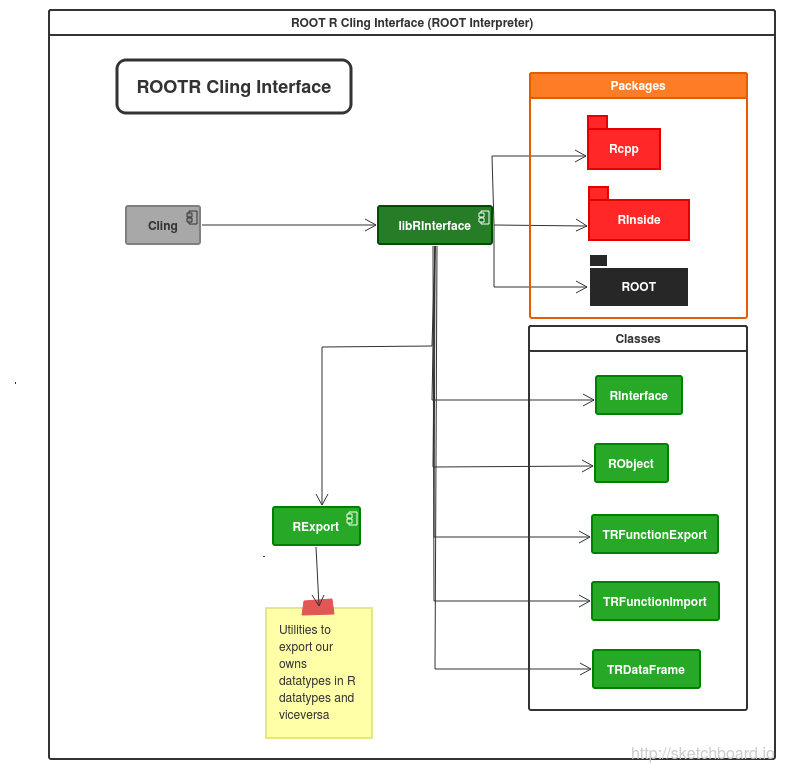
\includegraphics[width=25pc]{img/rootr.png}\caption{\label{rootr:label} ROOT-R design.}
\end{figure}


\section{TMVA}
TMVA is ROOT's toolkit for multivariate data analysis
that implements machine learning algorithms for
classification and regression.
It has a good set of algorithms widely used in HEP:
\begin{itemize}  
\item BDT(Boosted Decision Trees)
\item ANN(Artificial Neural Networks)
\item SVM(Support Vector Machine)
\item LDA(Linear discriminant analysis)
\item And more \ldots 
\end{itemize}
TMVA has now a new set of plugins that is using python and R interfaces for classification, lets see (Figure \ref{tmva:label})
It is explained in the  section \ref{RMVA} ROOT-R with TMVA and section \ref{PYMVA} Python with TMVA.

\begin{figure}[h]
\centering
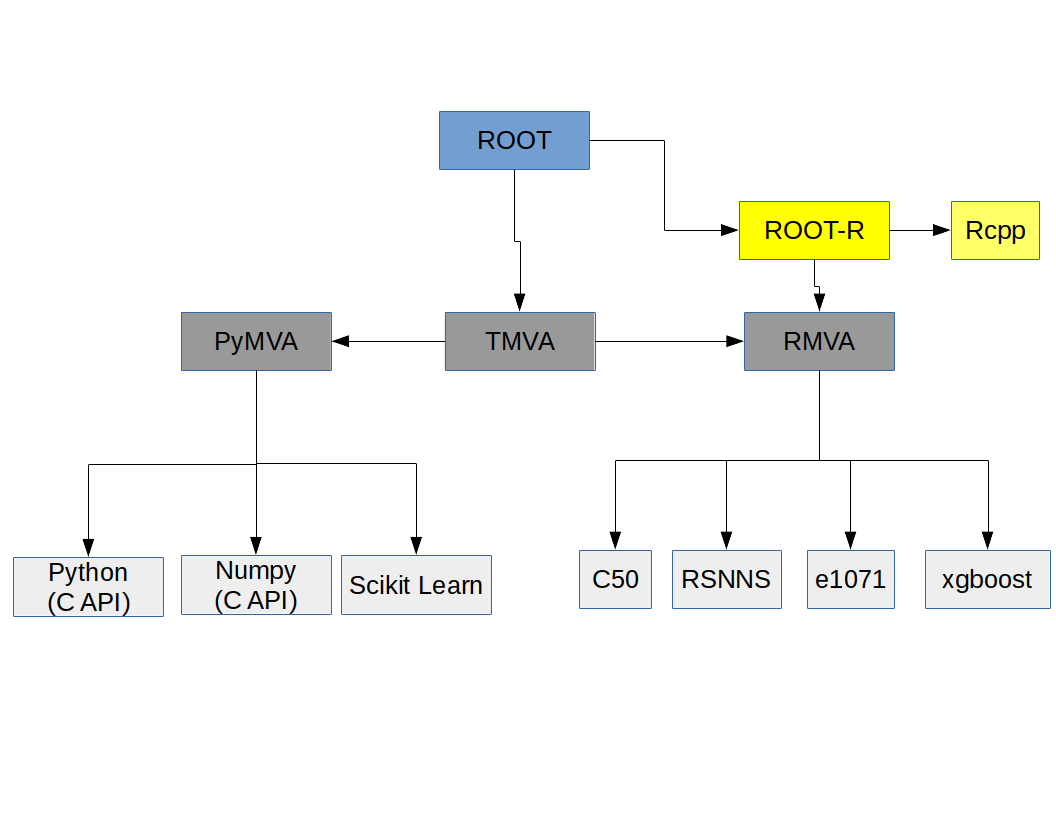
\includegraphics[width=25pc]{img/tmva.png}\caption{\label{tmva:label} Machine Learning Tools in ROOT.}
\end{figure}


\subsection{DataLoader}

TMVA DataLoader is a class that allows greater
modularity and flexibility for training different classifiers
with different features.

\begin{itemize}  
\item Every booked method can to have different dataset.(Figure \ref{dl1})
\item TMVA::DataLoader can load data from .root files and .csv (comma separated values) also is the class to add variables, spectators and targets. (Figure \ref{dl2})
\item The TMVA::DataLoader is the class that create TMVA::DataSet and TMVA::DataSetInfo for every method booked. (Figure \ref{dl3})
\item The class TMVA::DataLoader have a name that is a directory in the output file(.root). In these directory you can find the Train/Test data of the DataLoader.
\end{itemize}

\begin{figure}[h]
\begin{minipage}{15pc}
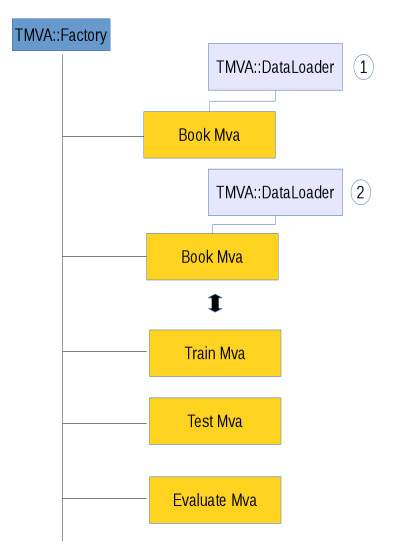
\includegraphics[width=15pc]{img/dl1.jpg}
\caption{\label{dl1}Booking methods with different dataloaders}
\end{minipage}\hspace{2pc}%
\begin{minipage}{15pc}
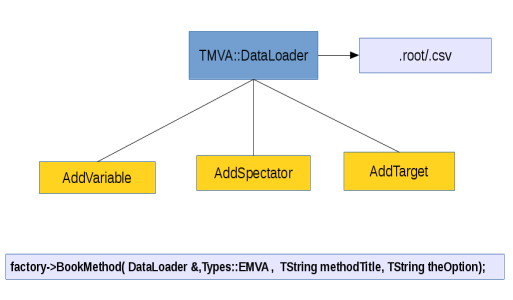
\includegraphics[width=15pc]{img/dl2.jpg}
\caption{\label{dl2}Loading data from files.}
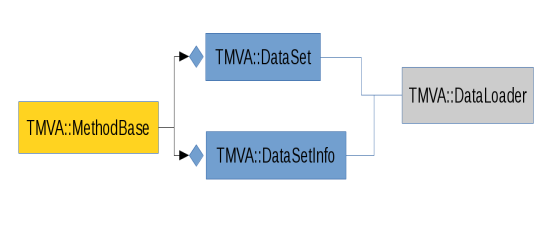
\includegraphics[width=15pc]{img/dl3.jpg}
\caption{\label{dl3}Loading data from files.}
\end{minipage} 
\end{figure}



\subsection{Variable Importance}
TODO
% Algorithm ranks the importance of a variable in
% classfication processes.
% \begin{itemize}  
% \item The method take a subset of variables and compute
% weights.
% \begin{itemize}  
% \item  Full variable set {V}
% \item Variable subset {S}
% \item Classifier Performance F(S)
% \end{itemize}  
% \item It is independent of the classifier.
% \item Is a stochastic algorithm.
% \end{itemize}  

\clearpage
\subsection{ROOT-R with TMVA}\label{RMVA}
RMVA is a set of plugins for TMVA package based on ROOTR
that allows new methods of classification and regression calling
R's packages.
Every method inherits from the base class RMethodBase (Figure \ref{rmvaplug})
to create a plugin and in the class RMethodBase is created some objects of TDataFrame class to map
the dataset from ROOT trees to dataframes in R.(Figure \ref{rmvadf}) 
\begin{itemize}  
\item (C50) C5.0 decision trees and rule-based models for pattern
recognition.
\item (RSNNS)Neural Networks in R using the Stuttgart Neural
Network Simulator (SNNS)
\item (e1071) Support Vector Machine can be used to carry out
general regression and classification (of nu and epsilon-type),
as well as density-estimation. A formula interface is provided.
\item eXtreme Gradient Boost (R package xgboost) An optimized
general purpose gradient boosting library.
\item It implements machine learning algorithms under the Gradient
Boosting framework, including Generalized Linear Model (GLM)
and Gradient Boosted Decision Trees (GBDT). 
\end{itemize}

We can to see the performance of the methods in the ROC Curve with a simple montecarlo simulation.(Figure \ref{rmvaroc})

\begin{figure}[h]
\centering
\begin{minipage}{15pc}
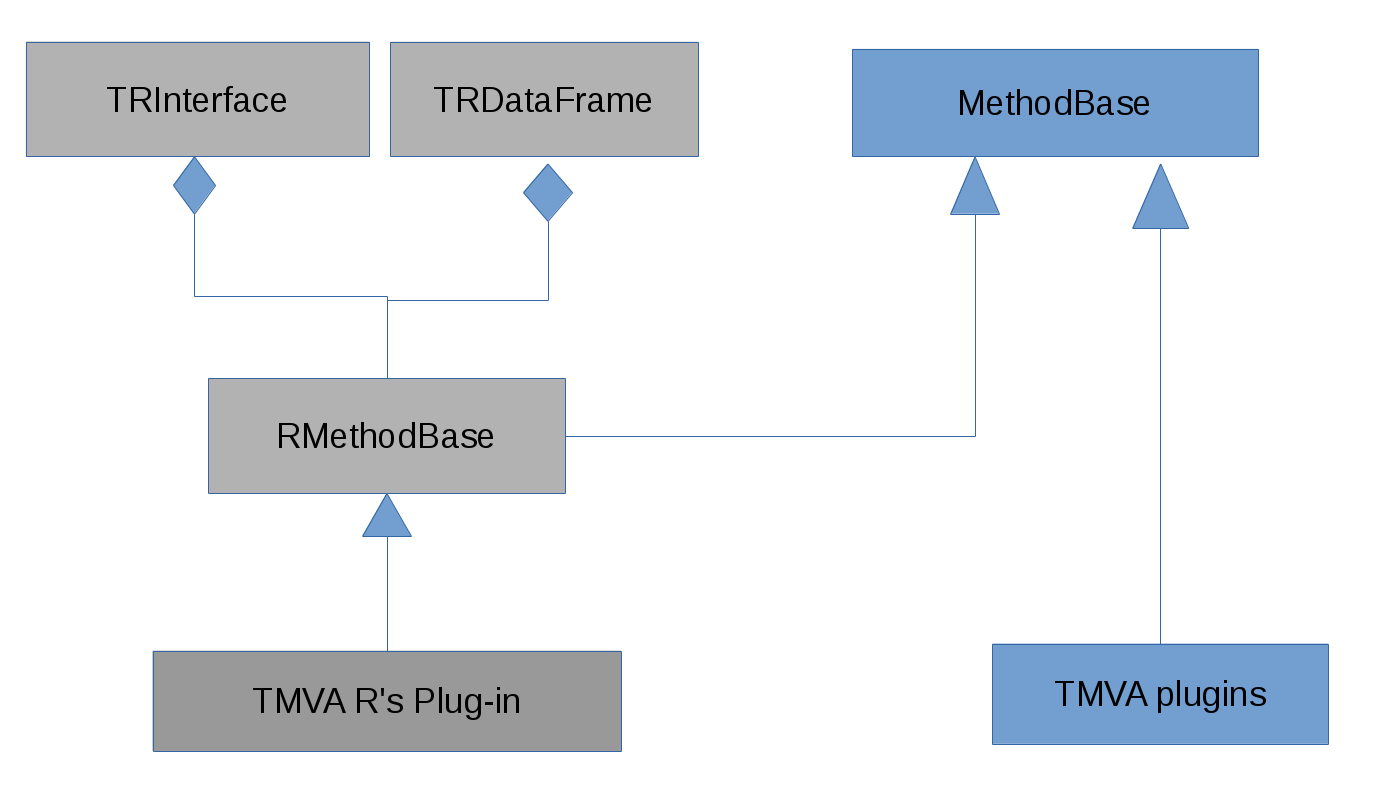
\includegraphics[width=16pc]{img/rmvaplugins.png}
\caption{\label{rmvaplug}ROOTR and TMVA plugins system}
\end{minipage}
\begin{minipage}{15pc}
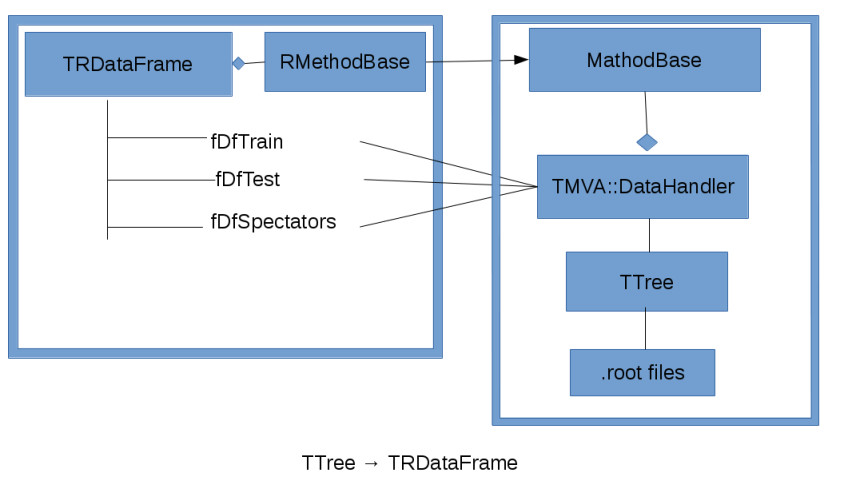
\includegraphics[width=16pc]{img/rmvadf.jpg}
\caption{\label{rmvadf}ROOTR and TMVA data flow.}
\end{minipage}\hspace{2pc}%
\end{figure}

\begin{figure}[h]
\centering
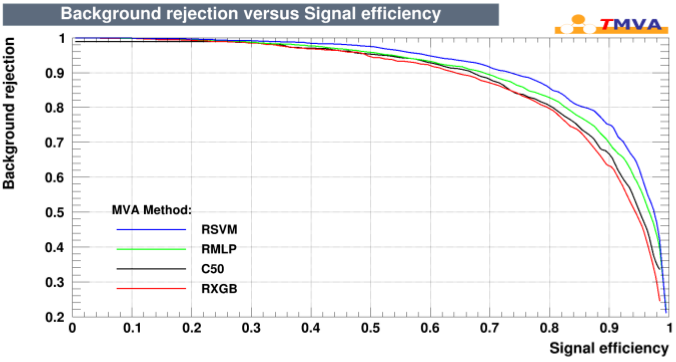
\includegraphics[width=25pc]{img/rmvaroc.png}\caption{\label{rmvaroc} ROC Curve for TMVA methods with ROOTR.}
\end{figure}

\clearpage
\subsection{Python with TMVA(Scikit Learn)} \label{PYMVA}
PyMVA is a set of TMVA plugins based on Python API that
allows new methods of classification and regression calling
Python's packages.

Every method inherits from the base class PyMethodBase (Figure \ref{pymvaplug})
to create a plugin and in the class PyMethodBase is created some objects of PyArrayObject class to map
the dataset from ROOT trees to numpy arrays in python.(Figure \ref{pymvadf}) 

Implemented Methods Based on Scikit-learn package
\begin{itemize}
\item PyRandomForest: in random forests each tree in the ensemble is built from a sample drawn with replacement (i.e., a bootstrap sample) from the training set.
\item PyGTB (Gradient Trees Boosted) : Gradient Tree Boosting or Gradient Boosted Regression Trees (GBRT) is a generalization of boosting to arbitrary differentiable loss
functions. GBRT is an accurate and effective off-the-shelf procedure that can be used for both regression and classification problems.
\item PyAdaBoost (Adaptative Boosting):The core principle of AdaBoost is to fit a sequence of weak learners (i.e., models that are only slightly better than random guessing, such as small
decision trees) on repeatedly modified versions of the data. 
\end{itemize}

We can to see the performance of the methods in the ROC Curve with a simple montecarlo simulation.(Figure \ref{pymvaroc})

\begin{figure}[h]
\centering
\begin{minipage}{15pc}
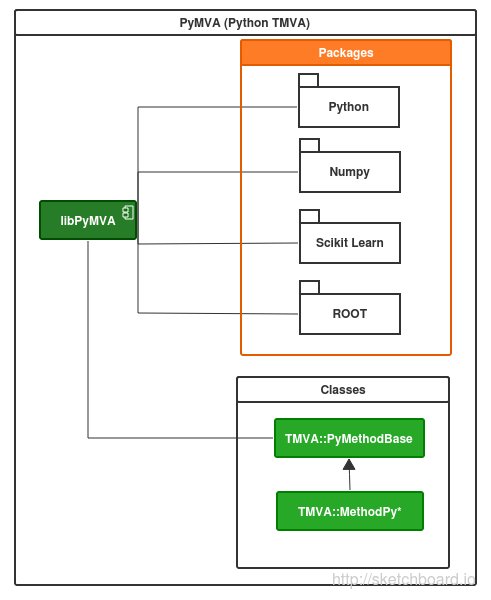
\includegraphics[width=16pc]{img/pymvaplugins.png}
\caption{\label{pymvaplug}Python and TMVA plugins system}
\end{minipage}\hspace{2pc}%
\begin{minipage}{15pc}
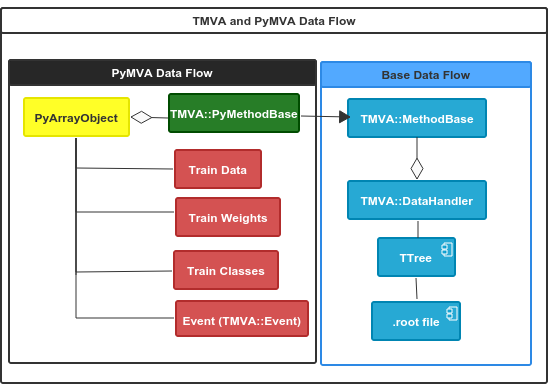
\includegraphics[width=16pc]{img/pymvadf.png}
\caption{\label{pymvadf}Python and TMVA data flow.}
\end{minipage}\hspace{2pc}%
\end{figure}

\begin{figure}[h]
\centering
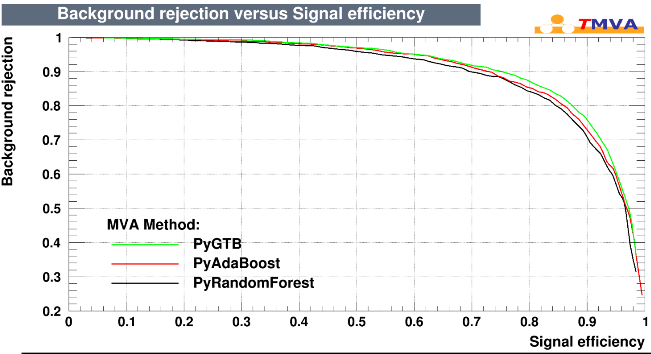
\includegraphics[width=25pc]{img/pymvaroc.png}\caption{\label{pymvaroc} ROC Curve for TMVA methods with Python.}
\end{figure}


\section{Incoming developments}
New TMVA::Factory design that allows more flexiblility to
integrate new techniques for:
\begin{itemize}
\item Cross validation
\item Data storage and manipulation (HDF5, CSV, JSON,
Custom Serialization FIles and SQL)
\item Improved design that will allow to use threads and new
parallelization technologies like OpenMP, MPI, cuda and
TBB.
\item New deep learning NN.
\item Improved Support Vector Machine 
\item  Additional deep learning plugins(deep belief nets and
restricted boltzmann machines)
\item Gaussian Processes
\end{itemize}

\subsection{Acknowledgments}
The work of Omar. A. Zapata has been partially supported by Sostenibilidad-UdeA, UdeA/CODI grant IN361CE
and COLCIENCIAS through the grant number 111-556-934918.
Computer Science Center, Metropolitan Institute of Technology - Medellin/Colombia.


\subsection{Appendices}
TODO


\section{References}
%%%%%%%%%%%%%%%%%%%%%%%%%%%%%%%%%%%%%%%%%%%
In the online version of \jpcs\ references will be linked to their original source or to the article within a secondary service such as INSPEC or ChemPort wherever possible. To facilitate this linking extra care should be taken when preparing reference lists. 

Two different styles of referencing are in common use: the Harvard alphabetical system and the Vancouver numerical system.  For \jpcs, the Vancouver numerical system is preferred but authors should use the Harvard alphabetical system if they wish to do so. In the numerical system references are numbered sequentially throughout the text within square brackets, like this [2], and one number can be used to designate several references.  

\subsection{Using \BibTeX}
We highly recommend the {\ttfamily\textbf\selectfont iopart-num} \BibTeX\ package by Mark~A~Caprio \cite{iopartnum}, which is included with this documentation.

\subsection{Reference lists}
A complete reference should provide the reader with enough information to locate the article concerned, whether published in print or electronic form, and should, depending on the type of reference, consist of:  

\begin{itemize}
\item name(s) and initials;
\item date published;
\item title of journal, book or other publication; 
\item titles of journal articles may also be included (optional);
\item volume number;
\item editors, if any;
\item town of publication and publisher in parentheses for {\it books};
\item the page numbers.
\end{itemize}

Up to ten authors may be given in a particular reference; where 
there are more than ten only the first should be given followed by 
`{\it et al}'. If an author is unsure of a particular journal's abbreviated title it is best to leave the title in 
full. The terms {\it loc.\ cit.\ }and {\it ibid.\ }should not be used. 
Unpublished conferences and reports should generally not be included 
in the reference list and articles in the course of publication should 
be entered only if the journal of publication is known. 
A thesis submitted for a higher degree may be included 
in the reference list if it has not been superseded by a published 
paper and is available through a library; sufficient information 
should be given for it to be traced readily.

\subsection{Formatting reference lists}
Numeric reference lists should contain the references within an unnumbered section (such as \verb"\section*{References}"). The 
reference list itself is started by the code 
\verb"\begin{thebibliography}{<num>}", where \verb"<num>" is the largest
number in the reference list and is completed by
\verb"\end{thebibliography}". 
Each reference starts with \verb"\bibitem{<label>}", where `label' is the label used for cross-referencing. Each \verb"\bibitem" should only contain a reference to a single article (or a single article and a preprint reference to the same article).  When one number actually covers a group of two or more references to different articles, \verb"\nonum"
should replace \verb"\bibitem{<label>}" at
the start of each reference in the group after the first.

For an alphabetic reference list use \verb"\begin{thereferences}" ... \verb"\end{thereferences}" instead of the
`thebibliography' environment and each reference can be start with just \verb"\item" instead of \verb"\bibitem{label}"
as cross referencing is less useful for alphabetic references.

\subsection {References to printed journal articles}
A normal reference to a journal article contains three changes of font (see table \ref{jfonts}) and is constructed as follows:

\begin{itemize}
\item the authors should be in the form surname (with only the first letter capitalized) followed by the initials with no periods after the initials. Authors should be separated by a comma except for the last two which should be separated by `and' with no comma preceding it;
\item the article title (if given) should be in lower case letters, except for an initial capital, and should follow the date;
\item the journal title is in italic and is abbreviated. If a journal has several parts denoted by different letters the part letter should be inserted after the journal in Roman type, e.g. {\it Phys. Rev.} A;
\item the volume number should be in bold type;
\item both the initial and final page numbers should be given where possible. The final page number should be in the shortest possible form and separated from the initial page number by an en rule `-- ', e.g. 1203--14, i.e. the numbers `12' are not repeated.
\end{itemize}

A typical (numerical) reference list might begin

\medskip
\begin{thebibliography}{9}
\item Strite S and Morkoc H 1992 {\it J. Vac. Sci. Technol.} B {\bf 10} 1237 
\item Jain S C, Willander M, Narayan J and van Overstraeten R 2000 
{\it J. Appl. Phys}. {\bf 87} 965 
\item Nakamura S, Senoh M, Nagahama S, Iwase N, Yamada T, Matsushita T, Kiyoku H 
and 	Sugimoto Y 1996 {\it Japan. J. Appl. Phys.} {\bf 35} L74 
\item Akasaki I, Sota S, Sakai H, Tanaka T, Koike M and Amano H 1996 
{\it Electron. Lett.} {\bf 32} 1105 
\item O'Leary S K, Foutz B E, Shur M S, Bhapkar U V and Eastman L F 1998 
{\it J. Appl. Phys.} {\bf 83} 826 
\item Jenkins D W and Dow J D 1989 {\it Phys. Rev.} B {\bf 39} 3317 
\end{thebibliography}
\smallskip

\noindent which would be obtained by typing

\begin{verbatim}
% \begin{\thebibliography}{9}
% \item Strite S and Morkoc H 1992 {\it J. Vac. Sci. Technol.} B {\bf 10} 1237 
% \item Jain S C, Willander M, Narayan J and van Overstraeten R 2000 
% {\it J. Appl. Phys}. {\bf 87} 965 
% \item Nakamura S, Senoh M, Nagahama S, Iwase N, Yamada T, Matsushita T, Kiyoku H 
% and 	Sugimoto Y 1996 {\it Japan. J. Appl. Phys.} {\bf 35} L74 
% \item Akasaki I, Sota S, Sakai H, Tanaka T, Koike M and Amano H 1996 
% {\it Electron. Lett.} {\bf 32} 1105 
% \item O'Leary S K, Foutz B E, Shur M S, Bhapkar U V and Eastman L F 1998 
% {\it J. Appl. Phys.} {\bf 83} 826 
% \item Jenkins D W and Dow J D 1989 {\it Phys. Rev.} B {\bf 39} 3317 
% \end{\thebibliography}
\end{verbatim}

\begin{center}
\begin{table}[h]
\centering
\caption{\label{jfonts}Font styles for a reference to a journal article.} 
\begin{tabular}{@{}l*{15}{l}}
\br
Element&Style\\
\mr
Authors&Roman type\\
Date&Roman type\\
Article title (optional)&Roman type\\
Journal title&Italic type\\
Volume number&Bold type\\
Page numbers&Roman type\\
\br
\end{tabular}
\end{table}
\end{center}

\subsection{References to \jpcs\ articles}
Each conference proceeding published in \jpcs\ will be a separate {\it volume}; 
references should follow the style for conventional printed journals. For example:\vspace{6pt}
\numrefs{1}
\item Douglas G 2004 \textit{J. Phys.: Conf. Series} \textbf{1} 23--36
\endnumrefs

%%%%%%%%%%%%%%%%%%%%%%%%%%%%%%%%%%
\subsection{References to preprints}
For preprints there are two distinct cases:
\renewcommand{\theenumi}{\arabic{enumi}}
\begin{enumerate}
\item Where the article has been published in a journal and the preprint is supplementary reference information. In this case it should be presented as:
\medskip
\numrefs{1}
\item Kunze K 2003 T-duality and Penrose limits of spatially homogeneous and inhomogeneous cosmologies {\it Phys. Rev.} D {\bf 68} 063517 ({\it Preprint} gr-qc/0303038)
\endnumrefs
\item Where the only reference available is the preprint. In this case it should be presented as
\medskip
\numrefs{1}
\item Milson R, Coley A, Pravda V and Pravdova A 2004 Alignment and algebraically special tensors {\it Preprint} gr-qc/0401010
\endnumrefs
\end{enumerate}

\subsection{References to electronic-only journals}
In general article numbers are given, and no page ranges, as most electronic-only journals start each article on page 1.

\begin{itemize} 
\item For {\it New Journal of Physics} (article number may have from one to three digits)
\numrefs{1}
\item Fischer R 2004 Bayesian group analysis of plasma-enhanced chemical vapour deposition data {\it New. J. Phys.} {\bf 6} 25 
\endnumrefs
\item For SISSA journals the volume is divided into monthly issues and these form part of the article number

\numrefs{2}
\item Horowitz G T and Maldacena J 2004 The black hole final state {\it J. High Energy Phys.}  	JHEP02(2004)008
\item Bentivegna E, Bonanno A and Reuter M 2004 Confronting the IR fixed point cosmology 	with 	high-redshift observations {\it J. Cosmol. Astropart. Phys.} JCAP01(2004)001  
\endnumrefs
\end{itemize} 

\subsection{References to books, conference proceedings and reports}
References to books, proceedings and reports are similar to journal references, but have 
only two changes of font (see table~\ref{book}). 

\begin{table}
\centering
\caption{\label{book}Font styles for references to books, conference proceedings and reports.}
\begin{tabular}{@{}l*{15}{l}}
\br
Element&Style\\
\mr
Authors&Roman type\\
Date&Roman type\\
Book title (optional)&Italic type\\
Editors&Roman type\\
Place (city, town etc) of publication&Roman type\\
Publisher&Roman type\\
Volume&Roman type\\
Page numbers&Roman type\\
\br
\end{tabular}
\end{table}

Points to note are:
\medskip
\begin{itemize}
\item Book titles are in italic and should be spelt out in full with initial capital letters for all except minor words. Words such as Proceedings, Symposium, International, Conference, Second, etc should be abbreviated to {\it Proc.}, {\it Symp.}, {\it Int.}, {\it Conf.}, {\it 2nd}, respectively, but the rest of the title should be given in full, followed by the date of the conference and the town or city where the conference was held. For Laboratory Reports the Laboratory should be spelt out wherever possible, e.g. {\it Argonne National Laboratory Report}.
\item The volume number, for example vol 2, should be followed by the editors, if any, in a form such as `ed A J Smith and P R Jones'. Use {\it et al} if there are more than two editors. Next comes the town of publication and publisher, within brackets and separated by a colon, and finally the page numbers preceded by p if only one number is given or pp if both the initial and final numbers are given.
\end{itemize}

Examples taken from published papers:
\medskip

\numrefs{99}
\item Kurata M 1982 {\it Numerical Analysis for Semiconductor Devices} (Lexington, MA: Heath)
\item Selberherr S 1984 {\it Analysis and Simulation of Semiconductor Devices} (Berlin: Springer)
\item Sze S M 1969 {\it Physics of Semiconductor Devices} (New York: Wiley-Interscience)
\item Dorman L I 1975 {\it Variations of Galactic Cosmic Rays} (Moscow: Moscow State University Press) p 103
\item Caplar R and Kulisic P 1973 {\it Proc. Int. Conf. on Nuclear Physics (Munich)} vol 1 (Amsterdam: 	North-Holland/American Elsevier) p 517
\item Cheng G X 2001 {\it Raman and Brillouin Scattering-Principles and Applications} (Beijing: Scientific) 
\item Szytula A and Leciejewicz J 1989 {\it Handbook on the Physics and Chemistry of Rare Earths} vol 12, ed K A Gschneidner Jr and L Erwin (Amsterdam: Elsevier) p 133
\item Kuhn T 1998 {\it Density matrix theory of coherent ultrafast dynamics Theory of Transport Properties of Semiconductor Nanostructures} (Electronic Materials vol 4) ed E Sch\"oll (London: Chapman and Hall) chapter 6 pp 173--214
\endnumrefs

\section{Tables and table captions}
Tables should be numbered serially and referred to in the text 
by number (table 1, etc, {\bf rather than} tab. 1). Each table should be a float and be positioned within the text at the most convenient place near to where it is first mentioned in the text. It should have an 
explanatory caption which should be as concise as possible. 

\subsection{The basic table format}
The standard form for a table is:
\begin{verbatim}
\begin{table}
\caption{\label{label}Table caption.}
\begin{center}
\begin{tabular}{llll}
\br
Head 1&Head 2&Head 3&Head 4\\
\mr
1.1&1.2&1.3&1.4\\
2.1&2.2&2.3&2.4\\
\br
\end{tabular}
\end{center}
\end{table}
\end{verbatim}

The above code produces table~\ref{ex}.

\begin{table}[h]
\caption{\label{ex}Table caption.}
\begin{center}
\begin{tabular}{llll}
\br
Head 1&Head 2&Head 3&Head 4\\
\mr
1.1&1.2&1.3&1.4\\
2.1&2.2&2.3&2.4\\
\br
\end{tabular}
\end{center}
\end{table}

Points to note are:
\medskip
\begin{enumerate}
\item The caption comes before the table.
\item The normal style is for tables to be centred in the same way as
equations. This is accomplished
by using \verb"\begin{center}" \dots\ \verb"\end{center}".

\item The default alignment of columns should be aligned left.

\item Tables should have only horizontal rules and no vertical ones. The rules at
the top and bottom are thicker than internal rules and are set with
\verb"\br" (bold rule). 
The rule separating the headings from the entries is set with
\verb"\mr" (medium rule). These commands do not need a following double backslash.

\item Numbers in columns should be aligned as appropriate, usually on the decimal point;
to help do this a control sequence \verb"\lineup" has been defined 
which sets \verb"\0" equal to a space the size of a digit, \verb"\m"
to be a space the width of a minus sign, and \verb"\-" to be a left
overlapping minus sign. \verb"\-" is for use in text mode while the other
two commands may be used in maths or text.
(\verb"\lineup" should only be used within a table
environment after the caption so that \verb"\-" has its normal meaning
elsewhere.) See table~\ref{tabone} for an example of a table where
\verb"\lineup" has been used.
\end{enumerate}

\begin{table}[h]
\caption{\label{tabone}A simple example produced using the standard table commands 
and $\backslash${\tt lineup} to assist in aligning columns on the 
decimal point. The width of the 
table and rules is set automatically by the 
preamble.} 

\begin{center}
\lineup
\begin{tabular}{*{7}{l}}
\br                              
$\0\0A$&$B$&$C$&\m$D$&\m$E$&$F$&$\0G$\cr 
\mr
\0\023.5&60  &0.53&$-20.2$&$-0.22$ &\01.7&\014.5\cr
\0\039.7&\-60&0.74&$-51.9$&$-0.208$&47.2 &146\cr 
\0123.7 &\00 &0.75&$-57.2$&\m---   &---  &---\cr 
3241.56 &60  &0.60&$-48.1$&$-0.29$ &41   &\015\cr 
\br
\end{tabular}
\end{center}
\end{table}
 
\section{Figures and figure captions}
Figures must be included in the source code of an article at the appropriate place in the text not grouped together at the end. 

Each figure should have a brief caption describing it and, if 
necessary, interpreting the various lines and symbols on the figure. 
As much lettering as possible should be removed from the figure itself and 
included in the caption. If a figure has parts, these should be 
labelled ($a$), ($b$), ($c$), etc. 
\Tref{blobs} gives the definitions for describing symbols and lines often
used within figure captions (more symbols are available
when using the optional packages loading the AMS extension fonts).

\begin{table}[h]
\caption{\label{blobs}Control sequences to describe lines and symbols in figure 
captions.}
\begin{center}
\begin{tabular}{lllll}
\br
Control sequence&Output&&Control sequence&Output\\
\mr
\verb"\dotted"&\dotted        &&\verb"\opencircle"&\opencircle\\
\verb"\dashed"&\dashed        &&\verb"\opentriangle"&\opentriangle\\
\verb"\broken"&\broken&&\verb"\opentriangledown"&\opentriangledown\\
\verb"\longbroken"&\longbroken&&\verb"\fullsquare"&\fullsquare\\
\verb"\chain"&\chain          &&\verb"\opensquare"&\opensquare\\
\verb"\dashddot"&\dashddot    &&\verb"\fullcircle"&\fullcircle\\
\verb"\full"&\full            &&\verb"\opendiamond"&\opendiamond\\
\br
\end{tabular}
\end{center}
\end{table}


Authors should try and use the space allocated to them as economically as possible. At times it may be convenient to put two figures side by side or the caption at the side of a figure. To put figures side by side, within a figure environment, put each figure and its caption into a minipage with an appropriate width (e.g. 3in or 18pc if the figures are of equal size) and then separate the figures slightly by adding some horizontal space between the two minipages (e.g. \verb"\hspace{.2in}" or \verb"\hspace{1.5pc}". To get the caption at the side of the figure add the small horizontal space after the \verb"\includegraphics" command and then put the \verb"\caption" within a minipage of the appropriate width aligned bottom, i.e. \verb"\begin{minipage}[b]{3in}" etc (see code in this file used to generate figures 1--3).

Note that it may be necessary to adjust the size of the figures (using optional arguments to \verb"\includegraphics", for instance \verb"[width=3in]") to get you article to fit within your page allowance or to obtain good page breaks.

\begin{figure}[h]
\begin{minipage}{14pc}

\includegraphics[width=14pc]{name.eps}
\caption{\label{label}Figure caption for first of two sided figures.}
\end{minipage}\hspace{2pc}%
\begin{minipage}{14pc}

\includegraphics[width=14pc]{name.eps}
\caption{\label{label}Figure caption for second of two sided figures.}
\end{minipage} 
\end{figure}

\begin{figure}[h]

\includegraphics[width=14pc]{name.eps}\hspace{2pc}%
\begin{minipage}[b]{14pc}\caption{\label{label}Figure caption for a narrow figure where the caption is put at the side of the figure.}
\end{minipage}
\end{figure}

Using the graphicx package figures can be included using code such as:
\begin{verbatim}
\begin{figure}
\begin{center}
\includegraphics{file.eps}
\end{center}
\caption{\label{label}Figure caption}
\end{figure}
\end{verbatim}

\section*{References}
\begin{thebibliography}{9}
\bibitem{iopartnum} IOP Publishing is to grateful Mark A Caprio, Center for Theoretical Physics, Yale University, for permission to include the {\tt iopart-num} \BibTeX package (version 2.0, December 21, 2006) with  this documentation. Updates and new releases of {\tt iopart-num} can be found on \verb"www.ctan.org" (CTAN). 
\end{thebibliography}

\end{document}


